\documentclass[a4paper]{article}

\usepackage[czech]{babel}
\usepackage[utf8]{inputenc}
\usepackage[T1]{fontenc}
\usepackage{outlines}
\usepackage[hidelinks]{hyperref}
\usepackage{csquotes}

\usepackage[left=1.5cm, text={18cm, 26cm}, top=1.8cm]{geometry}

\usepackage{graphicx}
\usepackage{float}
\usepackage[usenames, dvipsnames]{xcolor}

\hypersetup {
    unicode = true,
    pdfauthor = {Josef Škorpík, Martin Pech},
    pdftitle = {Simulační studie},
    pdfsubject = {IMS},
    pdfkeywords = {IMS Projekt, balistika, ShKH vz. 77 Dana},
    % pdfproducer = {},
    % pdfcreator = {pdfTeX}
}            

\newcommand{\logo} {
    
\includegraphics[scale=0.8, keepaspectratio]{fig/logo.pdf}
}

\renewcommand*{\ttdefault}{lmtt}

\pdfminorversion=7


\begin{document}

    \begin{titlepage}
        \begin{center}
            \logo
            \\\vspace{\stretch{0.382}}
            {\Huge Simulační studie}\\\medskip
            {\LARGE Implementace abstraktního modelu autobusové linky}\\\medskip
            {\large	Hromadná osobní přeprava}
            \vspace{\stretch{0.618}}
        \end{center}
        {\Large \today \hfill
        \begin{tabular}{l l}
            \textbf{Martin Pech} & \textbf{(\texttt{xpechm00})} \\
            Josef Škorpík & (\texttt{xskorp04})
        \end{tabular}}
    \end{titlepage}

    \newpage

	\section{Úvod}
    \label{sec:intro}

    Tématem projektu je implementace abstraktního modelu~\cite[snímek 10]{IMS_slides} autobusové linky. Projekt vznikl jako zápočtová práce do předmětu Modelování a simulace.
    Tento model si klade za cíl najít optimální počet dopravních prostředků (například autobusů), které je potřeba rezerovovat pro danou linku tak, aby nedocházelo k dlouhému čekání a najít optimální jízdní řád na základě zadaných parametrů o hustotě provozu a struktuře dané autobusové linky. Optimální počet autobusů i jízdní řád je vyhodnocován podle spokojenosti cestujících, která je ovlivněna několika faktory. Jelikož je tento simulační model~\cite[snímek 44]{IMS_slides} zacílen pouze na výše uvedené cíle, připouští výskyt pouze takových jevů, které přímo ovlivňují jeho chování. Tyto jevy jsou popsány v kapitole~\ref{subsec:conceptual_model_description}.
    Chování modelu bylo demonstrováno na základě existující Jihomoravské autobusové linky číslo 501. Výsledky experimentů byly porovnány se skutečnými jízdními řády.

        \subsection{Autoři a~původ faktů}
        \label{subsec:authors}

            Na implementaci projektu a~tvorbě technické zprávy spolupracovali studenti Fakulty informačních technologií Vysokého učení technického v~Brně, Martin Pech a~Josef Škorpík.
            
            Údaje o počtu zastávek, průměrné době mezi zastávkami a intervalech mezi výjezdy autobusů, které byly použity pro výchozí nastavení modelu, vychází z veřejně přístupných jízdních řádů uveřejněných na webu Integrovaného dopravního systému Jihomoravského kraje \cite{Jizdni_rad}. 
            Pravděpodobnost výskytu dopravní nehody byla spočítána na základě veřejně dostupných statistik pro rok 2020, které každoročně uveřejňuje Policie České republiky \cite{Accident_statistics} a podle informací poskytnutých Ministerstevm dopravy České republiky k říjnu roku 2020 \cite{Pocet_ridicaku}. Z těchto informací je možná získat následující data pro rok 2020:
            \begin{outline}
            	\1 Počet platných řidičských průkazů: \textbf{6 002 348}
            	\1 Počet dopravních nehod: \textbf{94 797}, z toho počet dopravních nehod s jedoucím nekolejovým vozidlem: \textbf{28 333}
            \end{outline}
            
            Pro výpočet pravděpodobnosti dopravní nehody bylo dále pro jednoduchost uvažováno, že se žádná osoba neúčastnila více než jedné nehody. Výsledná pravděpodobnost se na základě těchto dat dá spočítat jako podíl počtu řidičských oprávnění a počtu nehod nekolejových vozidel. Výsledná hodnota je rovna přibližně \textbf{1 : 212}, tedy \textbf{0.0047\%}.
            
            Výchozí údaje o dopravní zácpě byly zjištěny experimentálně. Na trase linky 501 momentálně dochází mezi zastávkami Ořechovská a Ústřední hřbitov k rekonstrukci dálničního nájezdu, což má za následek každodenní mnohakilometrové kolony vozidel mířících na dálnici D1 směrem od Vídně. Tyto dopravní komplikace ovlivňují i vybranou autobusovou linku. Jeden z řešitelů (Martin Pech) jezdí denně osobním automobilem po trase linky 501. Při čekání zapisoval dobu takto strávenou.
            Z údajů získaných o dopravě v tomto úseku, od počátku října do konce listopadu, v době dopravní špičky bylo následně zjištěno, že k zácpě došlo pokaždé a průměrná doba čekání, ke kterému docházelo, byla vypočtena jako \textbf{17 minut}.
            
            Mimo tento úsek dané linky byly hodnoty zpoždění pouze zanedbatelné a to jak ve špičce, tak mimo ni. Díky tomu bylo možné jednoduše určit výchozí pravděpodobnost výskytu zácpy. Pravděpodobnost výskytu zácpy při špičce je tedy možné vyjádřit jako poměr problémového úseku vůči celkovému počtu úseků. Výsledná pravděpodobnost je tedy~\textbf{$\frac{1}{6}$}. 
            
            Pro určení průměrného počtu cestujících na zastávkách bylo využito statistik \cite{Pocet_cestujicich} uvedených na portálu wikipedie.org. Podle tohoto zdroje provozoval v roce 2022 Dopravní podnik města Brna 328 autobusů určených pro městskou osobní dopravu. Tyto autobusy v roce 2022 přepravily 111,7 milionů cestujících. Výchozí použitý autobus a jeho kapacita odpovídá typu SOR CN 12 \cite{PSOR_CN_12}.
            
            Z těchto údajů vyplývá, že jeden autobus převeze průměrně 39 lidí za hodinu. Trasa linky číslo 501 trvá ve vybraném úseku 9 minut a jede průměrně 3$\times$ za hodinu. Během jedné jízdy autobus převeze průměrně 13 lidí. 
            Po rozpočítání tohoto počtu mezi 7 zastávek, zůstavají průměrně 2 lidi na zastávku.
            Tato statistika vychází z celoročních dat, tudíž jsou zde počítány jak spoje v dopravní špičce, tak i noční spoje, kde je nízké vytížení. Tento vypočtený údaj je pro daný model nedostatečný, ale nebylo možné vyhledat lepší údaje. Ze zkušenosti jednoho z řešitelů je ale průměrný počet lidí na zastávce mnohem vyšší, zejména ve špičce.

        \subsection{Validace výstupů}
        \label{subsec:validation}
        V rámci validace výstupů bylo provedeno několik experimentů (popsané v kapitole \ref{sec:simulation}) a výsledky těchto experimentů byly validovány s daty z původního jízdního řádu a nového výlukového jízdního řádu, který Integrovaný dopravní systém vytvořil v reakci na situace mezi zastávkami Ořechovská a Ústřední hřbitov. 
	
\newpage
    \section{Rozbor tématu a~použitých metod/technologií}
    \label{sec:methods}
   		Tento model hromadné osobní přepravy se zaměřuje na nalezení optimálního jízdního řádu autobusové linky. Model vyhodnocuje vstupní parametry, ze kterých určuje výsledky. Výstupy modelu jsou určovány na základě spokojenosti pasažérů. Spokojenost pasažérů je určována na základě běžných situací, jako například čekání v koloně, opožděný a včasný příjezd, nebo situace, kdy je autobus přeplněný a nemohou do něj nastoupit další lidé. Pro určení míry spokojenosti a nespokojenosti jednotlivých aspektů bylo využito dotazníkového šetření. Dotazovaní měli za úkol určit míru spokojenosti a nespokojenosti u každého z použitých aspektů. Po zprůměrování všech výsledků je spokojenost ovlivňována následujícími aspekty s následující váhou (za každého jednoho pasažéra, kterého se situace týká): 
   		
         \begin{table}[H]
   			\centering
   			\resizebox{\textwidth}{!}{
   				\begin{tabular}{ | c | c | c | c | c | c | c | c| }
   					\hline
   					Zpožděný přijezd autobusu & Včasný příjezd autobusů &  Přeplněný autobus & Čekání v dopravní zácpě & Opožděný příjezd autobusu do zastávky & Dopravní nehoda \\
   					\hline
   					\hline
   					-1/-2 & +1/+2 & -1/-2 & 0/-1 & 0/-1 & -3 \\
   					\hline
   				\end{tabular}
   			}
   			\caption{Ovlivnění celkové spokojenosti v závislosti na daném jevu (za každého jednoho pasažéra). Každý aspekt má jednu až dvě hodnoty. V případě dvou hodnot je konkrétní hodnota vybrána z dostupných variant náhodně pro každého pasažéra.}
   			\label{}
   		\end{table}
   		
     	Po nasimulování autobusové linky s konkrétními parametry je uživatel obeznámen s výsledkem. Pokud je výsledek spokojenosti pasažérů nadprůměrný, znamená to, že by takovýto jízdní řád za daných podmínek mohl fungovat. Model dále dokáže indikovat situaci, kdy je na lince použitý nesprávny počet autobusů, což může vést k ekonomické neúnosnosti, nebo jsou intervaly mezi výjezdy autobusů příliš (málo) četné. Dále dokáže určit taková nastavení, která by v reálném provozu zřejmě neobstála.
   		
   		Výchozí nastavení modelu odpovídá autobusové lince 501. Pomocí jízdního řádu této linky byl následně model validován. 
 		Model uvažuje všechny autobusové zastávky od Ústředního hřbitova po Nebovidy, dolní konec. V tomto úseku je 7 autobusových zastávek a celková doba jízdy autobusu po této trase (bez zpoždění) je 9 minut. Simulační čas odpovídá minutám reálného času. 
 		
 		Chování modelu je takové, že po pevně daných časových intervalech vyjíždí z úvodní zastávky autobus a projíždí všechny zastávky na lince. Mezi všemi zastávkami na lince existuje šance, že se autobus dostane do dopravní zácpy, v důsledku čehož se opozdí. To může mít negativní dopad na schopnost autobusu vyjet na novou linku podle jízdního řádu, čímž se může negativně ovlivňovat spokojenost pasažérů. Pokud autobus přijede k zastávce, existuje možnost, že se v zastávce vyskytuje už nějaký jiný autobus. V takovém případě se autobus zařadí do fronty na zastávku. V opačném případě zabere zastávku a započne výstup a nástup cestujících. Pokud je kapacita autobusu zaplněna, nejsou další cestující vpuštěni do autobusu, což znovu negativně ovlivňuje jejich spokojenost. Po dokončení zastávky se autobus vrací na silnici. V tomto momentě hrozí riziko nedání přednosti v jízdě, ze strany řidičů, a s šancí 0,0047\% může dojít k nehodě.
 		V takovém případě se na linku vysílá náhradní autobus, který převezme všechny cestující z havarovaného autobusu a pokračuje dál na lince. Nabouraný autobus již není možné použít.
 		
 		Z výše popsaných dat vyplývá, že se průměrně na každé zastávce vyskytují 2 lidé. Obdobně uvažujeme i počet vystupujících. Obecně ale platí, že se cestující generují s rovnoměrným rozložením, daným intervalem <0, x>, kde x může uživatel nastavit přepínačem jak pro nástup, tak pro výstup. Výchozí hodnota je pro oba případy $x = 4$. Výjimkou je poslední zastávka, kde se implicitně uvažuje výstup všech cestujících.
 		Naložení a vyložení cestujících trvá průměrně 1,5 minuty. Průměrný čas mezi jednotlivými zastávkami na této lince je 1,3 minuty. 
 		Ve výchozím nastavení vyjíždí nový autobus každých 11,25 minut a k dispozici jsou tři autobusy s kapacitou 75 míst.  Všechny v této kapitole popsané parametry lze modifikovat pomocí argumentů příkazové řádky při spouštění modelu.
     
        \subsection{Popis použitých postupů}
        \label{subsec:methods}

            K vytvoření základní koncepce projektu bylo využito deklarativních modelů~\cite[snímek 49]{IMS_slides}, konkrétně Petriho sítě~\cite[snímek 123]{IMS_slides} vyobrazené níže.
            Pomocí Petriho sítí byl vytvořen model obslužné linky, simulující chování linky hromadné osobní přepravy. Model byl vytvořen za pomoci progamovacího jazyka C++, který je velmi dobře využitelný v případech, kdy je nutný vysoký výkon. Proto je ideální volbou pro tvorbu simulací, které mohou být výpočetně náročné. Pro účely modelování je využito knihovnu SIMLIB \footnote{\url{https://www.fit.vutbr.cz/~peringer/SIMLIB/}} ve verzi 3.09 a pro sestavení projektu nástroje GNU Make \footnote{\url{https://www.gnu.org/software/make/}}. Nástroj i knihovna jsou volně dostupné a jsou distribuovány pod svobodnou licencí softwaru.
            
        \subsection{Popis původu použitých metod/technologií}
        \label{subsec:techology}

			S~pomocí jazyka C++ bylo přistupováno k~rozhraní knihovny SIMLIB, pomocí kterého byly vytvořeny předpisy pro všechny komponenty potřebné k~simulaci. Díky principům jazyka C++ bylo možné využít objektově orientovaného programování. Proces autobusu byl implementován ve třídě Bus a proces dopravní nehody ve třídě Accident.

    \section{Koncepce modelu}
    \label{sec:concept}

        Konceptuální model~\cite[snímek 48]{IMS_slides} je koncipován jako systém hromadné obsluhy~\cite[snímek 136]{IMS_slides}.
        V modelu se pracuje s obslužnou linkou autobusu, která zpracovává příchozí požadavky na výjezd autobusu dle jízdního řádu. Dále v modelu existuje dynamický počet linek reprezentující autobusové zastávky. Počet zastávek volí uživatel při spouštění programu. Díky tomu, že se tento model neomezuje na počet autobusových zastávek, či na předem daný počet autobusů, je možné ho použít k modelování libovolné linky. V modelu se dále vyskytuje dispečer, který pravidelně vysílá autobusy.

        \subsection{Popis konceptuálního modelu}
        \label{subsec:conceptual_model_description}
            Do modelu vstupují jednotlivé autobusy v pevně daných intervalech. 
            V čas výjezdu vyjíždí autobus na první zastávku. Na zastávce nabírá cestující. Mohou nastat dvě komplikace. Autobus může havarovat, na základě čehož vyšle systém nový autobus na místo havárie. Nový autobus převezme cestující a poté pokračuje v dané lince namísto původního autobusu. Druhou komplikací je dopravní zácpa, do které se autobus může dostat. Výstupem modelu je spokojenost cestujících a statistiky o průměrném zpoždění a počtu využitých autobusů. Spokojenost je ovlivněna časem příjezdu do cílové destinace a dalšími faktory. Pokud cestující přijede bez komplikací a včas, dá se říct, že byl se službou dané linky spokojený. Pokud se dostane do havárie nebo dopravní zácpy,dá se očekávat, že cestující nebude se službou spokojen.
            
        \subsection{Forma konceptuálního modelu}
        \label{subsec:conceptual_model}

            Model je reprezentován následující Petriho sítí.

            \begin{figure}[H]
                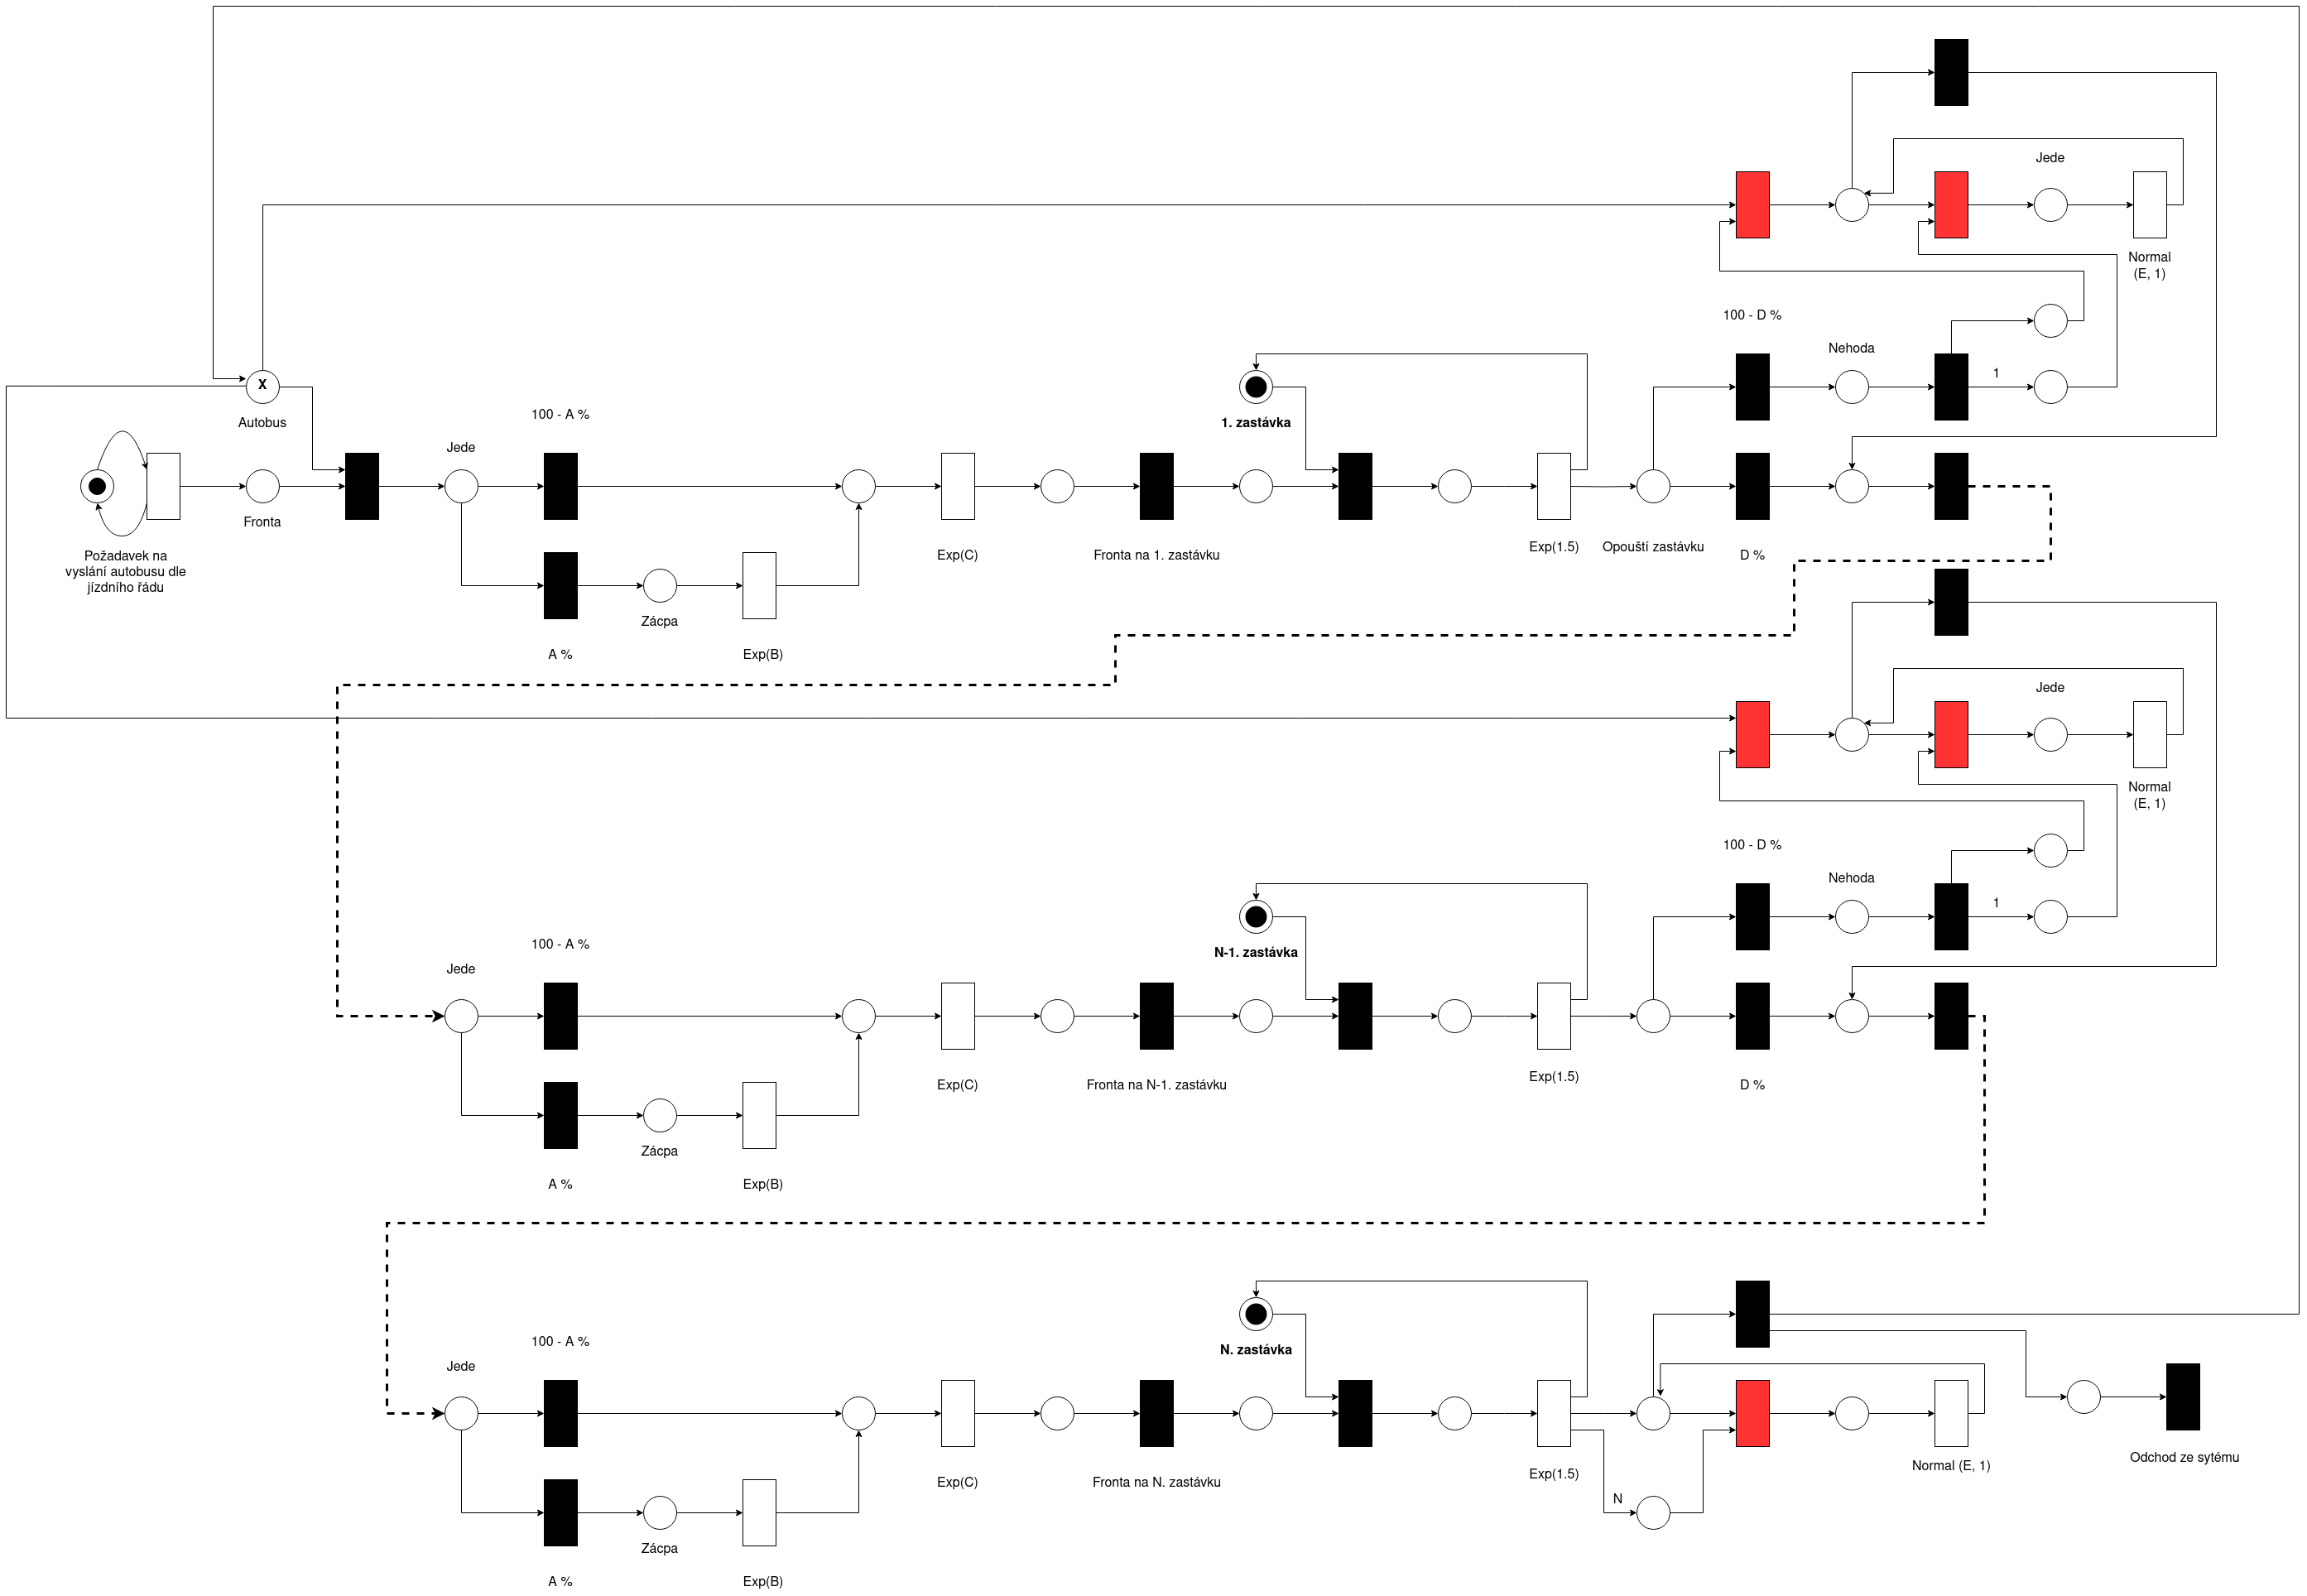
\includegraphics[scale=0.18, keepaspectratio]{fig/petri_doprava.png}
                \caption{Petriho síť}
                \label{fig:petri_nest}
            \end{figure}

            \begin{table}[H]
                \centering
                \begin{tabular}{ l l }
                    $X$ & Kapacita linky autobusu \\
                    $N$ & N-tá linka reprezentující autobusovou zastávku o kapacitě 1 \\
                    $A$ & Pravděpodobnost dopravní zácpy \\
                    $B$ & Doba čekání v zácpě dané exponenciálním rozložením se zadaným středem \\
                    $C$ & Doba přejezdu do další zastávky dané exponenciálním rozložením se zadaným středem \\
                    $D$ & Pravděpodobnost nehody \\
                    $E$ & Reprezentuje dobu přejezdu mezi zastávkami \\
                    \textit{Červené bloky} & Znázorňují zvýšenou prioritu přechodu, priorita = 1\\
                    \textit{Bílé bloky} & Znázorňují časové přechody\\
                    \textit{Černé bloky} & Znázorňují funkční/nečasové přechody\\
                \end{tabular}
                \caption{Legenda k~Petriho síti}
                \label{tab:petri}
            \end{table}


    \section{Architektura simulačního modelu}
    \label{sec:architecture}

        Spuštěním simulačního modelu~\cite[snímek 44]{IMS_slides} se spustí simulační experiment se zadanými parametry.
        Parametry a jejich zadávání jsou popsány v~kapitole~\ref{subsec:start}. Během simulačního experimentu jsou vypisovány všechny podstatné změny stavů.
        Výpis každé změny stavu je doprovázen modelovým časem~\cite[snímek 21]{IMS_slides}. Modelový čas odpovídá minutám reálného času. Příkladem změny stavu může být například to, že se autobus dostal do havárie, nebo to, že se na místo havárie vyslal nový autobus. Stavy a jejch přechody jsou znázorněny v~Petriho síti v~kapitole~\ref{subsec:conceptual_model}.

		Pro účely simulace byl simulační čas nastaven na 1 hodinu a 40 minut. Tato doba byla určena na základě jízdního řádu. Jízdnímu řádu odpovídají i intervaly, po kterých je vygenerován požadavek na vyslání autobusu a doba jeho přesunu mezi zastávkami.

        Modelový čas~\cite[snímek 21]{IMS_slides} lze nastavit způsobem popsaným v~kapitole~\ref{subsec:start}. Jednotka modelového času je chápána jako
        minuta v~reálném čase.
        Model dále pracuje s~5~\%~šancí , že se autobus dostane do dopravní zácpy, ve které průměrně strávi 5 minut a s 0.00471\% šancí, že autobus havaruje.

        \subsection{Mapování konceptuálního modelu do simulačního modelu}
        \label{subsec:mapping}

            Generování požadavků na vypravení autobusu je reprezentováno třídou \texttt{BusDispatcher}, která je implementována jako
            událost~\cite[snímek 172]{IMS_slides}. Proces~\cite[snímek 174]{IMS_slides} chování autobusu je implementován třídou \texttt{Bus}. Dalším samostatným procesem je nehoda, která je reprezentována třídou \texttt{Accident}. V konceptuálním modelu se vyskytují fronty~\cite[snímek 141]{IMS_slides}, které jsou implementovány pomocí třídy Queue z knihovny Simlib. Dále se vyskytují obslužné linky~\cite[snímek 62]{IMS_slides}, které je možné zabírat, nebo k nim prioritně přistupovat. Linky jsou implementovány pomocí třídy Facility z knihovny Simlib.

        \subsection{Spouštění simulačního modelu}
        \label{subsec:start}

            Simulační experiment je možné spouštět s~parametry, které ovlivňují jeho chování. Pokud není zadán žádný parametr, použijí se výchozí hodnoty pro linku číslo 501.
            
            \begin{itemize}
                \item Parametr \texttt{-t}  nastavit modelový čas, jeho výchozí hodnota je 100 minut a jeho hodnota musí vždy být kladné číslo.
                \item Parametr \texttt{-a} umožňuje nastavit pravděpodobnost, s jakou se autobus dostane do havárie. Hodnota parametru musí být kladné číslo v intervalu <0,1>.
                \item Parametr \texttt{-b} umožňuje nastavit počet autobusů, které operují na dané lince hromadné dopravy. Výchozí hodnota je 2. Hodnota musí být kladné celé číslo.
                \item Parametr \texttt{-s} umožňuje nastavit počet autobusových zastávek na dané lince. Výchozí hodnota je 7. Hodnota musí být kladné celé číslo.
                \item Parametr \texttt{-l} umožňuje nastavit pruměrný čas mezi jednotlivými autobusovými zastávkami. Výchozí hodnota je 1,3 minuty. Hodnota musí být kladné číslo.
                \item Parametr \texttt{-g} umožňuje nastavit interval, ve kterém vyjíždí jednotlivé autobusy. Výchozí hodnota je 11,25 minut. Hodnota musí být kladné číslo.
                \item Parametr \texttt{-w} umožňuje nastavit čas, který průměrně autobus stráví v dopravní zácpě. Výchozí hodnota je 5 minut. Hodnota musí být kladné číslo.
                \item Parametr \texttt{-j} umožňuje měnit šanci, se kterou se autobus dostane do dopravní zácpy. Výchozí hodnota je nastavena na 0.00471\%. Parametr musí být kaldné číslo v intervalu <0,1>.
                \item Parametr \texttt{-c} umožňuje nastavit kapacitu cestujících autobusu. Výchozí hodnota je 75 cestujících. Hodnota musí být kladné  celé číslo.
            
            \item Parametr \texttt{-i} umožnuje nastavit pravou hranici intervalu <0,x> rovnoměrného rozložení, podle kterého se určuje počet cestujících čekajících na zastávce. Hodnota musí být kladné celé číslo.
            \item Parametr \texttt{-o} umožnuje nastavit pravou hranici intervalu <0,y> rovnoměrného rozložení, podle kterého se určuje počet cestujících, kteří vystoupí z autobusu na zastávce. Hodnota musí být kladné celé číslo.
            \item Parametr \texttt{-r} umožňuje znáhodnodťovat jevy nastavením náhodné hodnoty do prvního prvku pseudonáhodného generátoru~\cite[snímek 72]{IMS_slides}. 
            \end{itemize}

            Program s~výchozími hodnotami je možné spustit příkazem \texttt{make run}.

    \section{Podstata simulačních experimentů a~jejich průběh}
    \label{sec:simulation}

        Cílem experimentů bylo pozorovat chování modelu a vytvořit závěry ohledně zvolené autobusové linky. Pozorováním modelu bylo možné dojít k závěrům ohledně aktuální situace na dané lince.
        \subsection{Postup experimentování}
        \label{subsec:experiments_methods}
			Experimentování probíhalo tak, že byly na základě jízdních řádů spočítány vstupní hodnoty pro několik situací. Výsledky z experimentů byly po dokončení validovány se skutečností.

            Experiment každé jedné situace byl spouštěn se zvolenými parametry, které jsou zaneseny v tabulkách níže. Nejsou--li v tabulce některé parametry uvedeny, byla uvažována jejich implicitní hodnota. Průběh každého experimentu je doplněn o snímek s výstupem z implementovaného modelu.
        \subsection{Experimenty}
        \label{subsec:experiments}

            Každý experiment má svůj dílčí cíl a závěr a nachází se u něj výpis jeho výsledků. Výsledky všech experimentů dohromady utváří celkový výsledek. Vysvětlení intervalů v tabulkách níže:
            \begin{itemize}
            	\item Interval nástupu - Reprezentuje počet cestujících nastupujících na jedné zastávce, je intervalem rovnoměrného rozdělení 
            	
            	\item Interval výstupu - Reprezentuje počet cestujících vystupujících na jedné zastávce, je intervalem rovnoměrného rozdělení 
            	
            	\item Čas mezi zastávkami je vždy vypočítán Exponenciální rozdělení s parametrem $\lambda$ = zadaná tabulková hodnota 
            	
            	\item Čas v dopravní zácpě je vždy vypočítán Exponenciální rozdělení s parametrem $\lambda$ = zadaná tabulková hodnota 
            \end{itemize}
			\newpage
            \subsubsection{Experiment 1}
            \label{subsubsec:experiment1}

                Cílem tohoto experimentu bylo ověření funkčnosti modelu s výchozími vstupy a získání doporučení ohledně jízdního řádu zvolené linky mimo dopravní špičku.

                \begin{table}[H]
                    \centering
                    \resizebox{\textwidth}{!}{
                    \begin{tabular}{ | c | c | c | c | c | c | c | c| }
                        \hline
                         Celkový čas (min) & Počet autobusů &  Počet zastávek & Průměrný čas mezi zastávkami (min) & Šance na dopravní zácpu & Čas v dopravní zácpě (min) & Šance na havárii & Spokojenost\\
                        \hline
                        \hline
                        100 & 2 & 7 & 1,3 & 5\% & 5 & 0.00471\% & \textcolor[rgb]{0,0.5,0}{Nadprůměrná}\\
                        \hline
                    \end{tabular}
                    }
                    \caption{Výsledek experimentu 1}
                    \label{tab:experiment1}
                \end{table}

				Z výsledku je patrné, že pro zadané parametry by mohl být výstup optimální. Hlavní znaky optimálního výsledku jsou spokojenost pasažérů a nízké opoždění autobusů. Dále model říká, že z dostupných autobusů využil všechny a tím pádem je i z hlediska využití dostupných zdrojů optimální. Dále je z podrobných výpisů změn stavů patrné, že se některý z autobusů dostal do dopravní zácpy.

                \begin{figure}[H]
                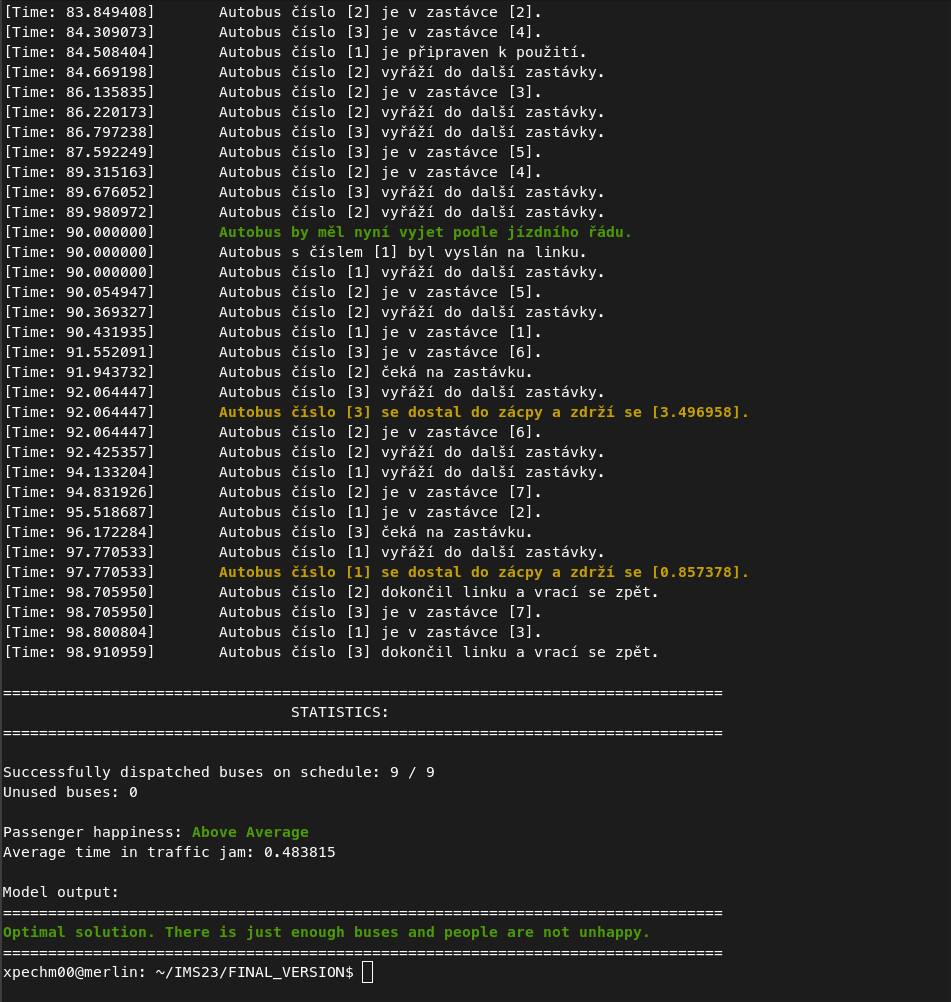
\includegraphics[scale=0.45, keepaspectratio]{fig/ims_bus1.png}
                \caption{Experiment 1 - mimo dopravní špičku}
                \label{fig:experiment1}
            \end{figure}
        \newpage
            \subsubsection{Experiment 2}
            \label{subsubsec:experiment2}
				Tento experiment se zaměřuje na situaci, kdy se zvolená autobusová linka nachází v dopravní špičce se zachováním původního jízdního řádu. V dopravní špičce je zvýšená pravděpodobnost dopravní komplikace a je řádově více lidí, kteří potřebují nastoupit.

                \begin{table}[H]
                    \centering
                    \resizebox{\textwidth}{!}{
                    \begin{tabular}{ | c | c | c | c | c | c| c |}
                        \hline
                        Šance na dopravní zácpu & Interval nástupu & Interval výstupu & Doba strávená v zácpe (min) & Průměrný čas mezi zastávkami (min)& Šance na havárii & Spokojenost \\
                        \hline
                        \hline
                        14\% & <0,20> &<0,2>& 17 & 1,4 & 1\%  & \textcolor{red}{Podprůměrná}\\
                        \hline
                    \end{tabular}
                    }
                    \caption{Parametry experimentu 2}
                    \label{tab:experiment2}
                \end{table}

				Experiment dokázal, že je situace za dopravní špičky diametrálně odlišná a je potřeba ji řešit. Na základě výstupů je vidět, že pasažéři nebyli spokojeni. Z výstupů lze vyvodit, že je tato situace způsobena faktem, že drtivá většina autobusů vyrazila opožděná (musela čekat na obsluhu). Situace vznikla tak, že autobusy dlouho stály v dopravní zácpě a nestíhaly včas vyrazit na novou cestu.
                
                Model pro tuto situaci doporučuje upravit jízdní řád snížením intenzity požadavků, nebo zvýšit počet autobusů na lince.

                \begin{figure}[H]
                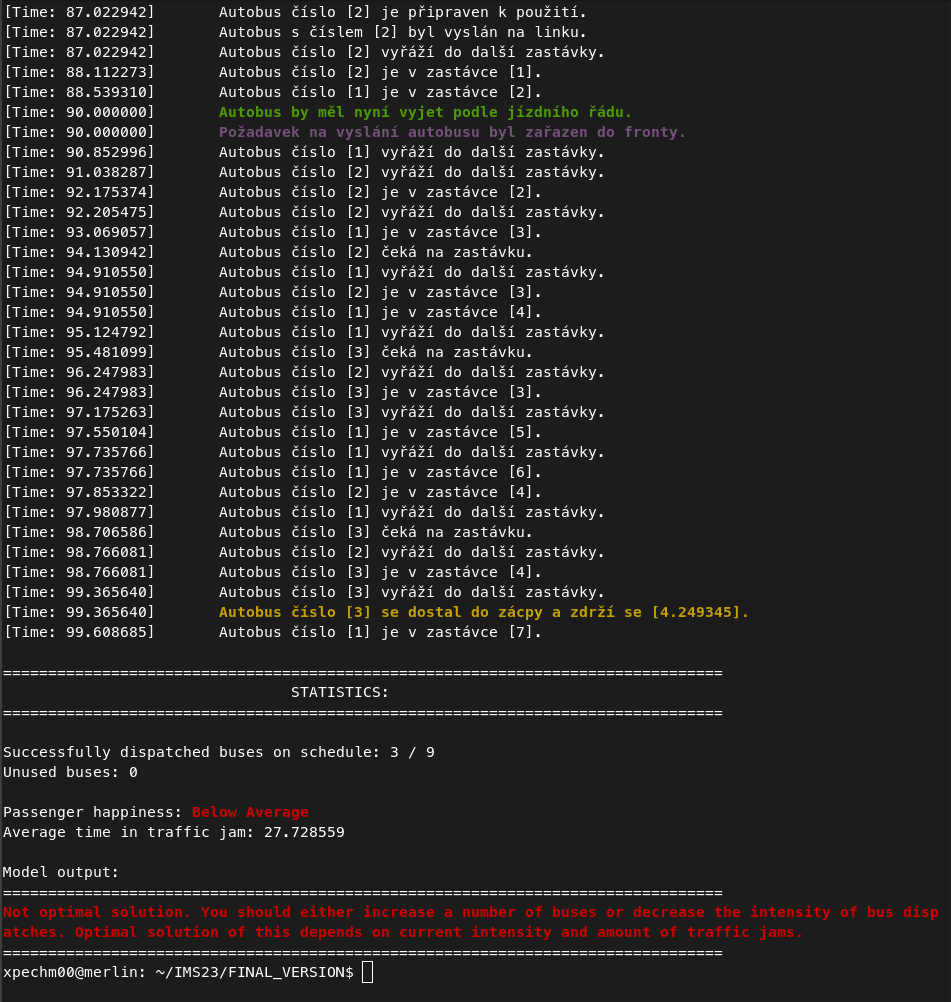
\includegraphics[scale=0.48, keepaspectratio]{fig/ims_bus2.png}
                \caption{Výsledek experimentu 2 - dopravní špička}
                \label{fig:experiment2}
            \end{figure}
    \newpage
            \subsubsection{Experiment 3}
            \label{subsubsec:experiment3}

				Na základě předchozího experimentu, jehož výsledek je patrný na obrázku \ref{tab:experiment2} je potřeba změnit jízdní řád. Trasa linky 501 umožňuje vynechat problémový úsek mezi zastávkami Ořechovská a Ústřední hřbitov, protože na zastávce Ořechovská je možné přesoupit na tramvaj. Parametry experimentu byly nastaveny tak, aby model simuloval chování autobusů na této \enquote{zkrácené lince}.
                

                \begin{table}[H]
                    \centering
                     \resizebox{\textwidth}{!}{
                    \begin{tabular}{ | c | c | c | c | c | c | c |}
                        \hline
                        Počet zastávek & Interval nástupu &  Interval výstupu &  Průměrný čas mezi zastávkami (min) & Šance na havárii & Spokojenost\\
                        \hline
                        \hline
                        6 & <0,20> & <0,2> & 1,4 &1\% & \textcolor[rgb]{0,0.5,0}{Nadprůměrná}\\
                        \hline
                    \end{tabular}
                    }
                    \caption{Parametry experimentu 3}
                    \label{tab:experiment3}
                \end{table}

            

                Model vyhodnotil \enquote{zkrácenou linku} jako fungující i v dopravní špičce. Tím pádem by takovýto jízdní řád bylo možné použít. S odkazem na jízdní řád \cite{Jizdni_rad} lze usoudit, že se ve skutečnosti této zkrácené linky opravdu využívá. 

                \begin{figure}[H]
                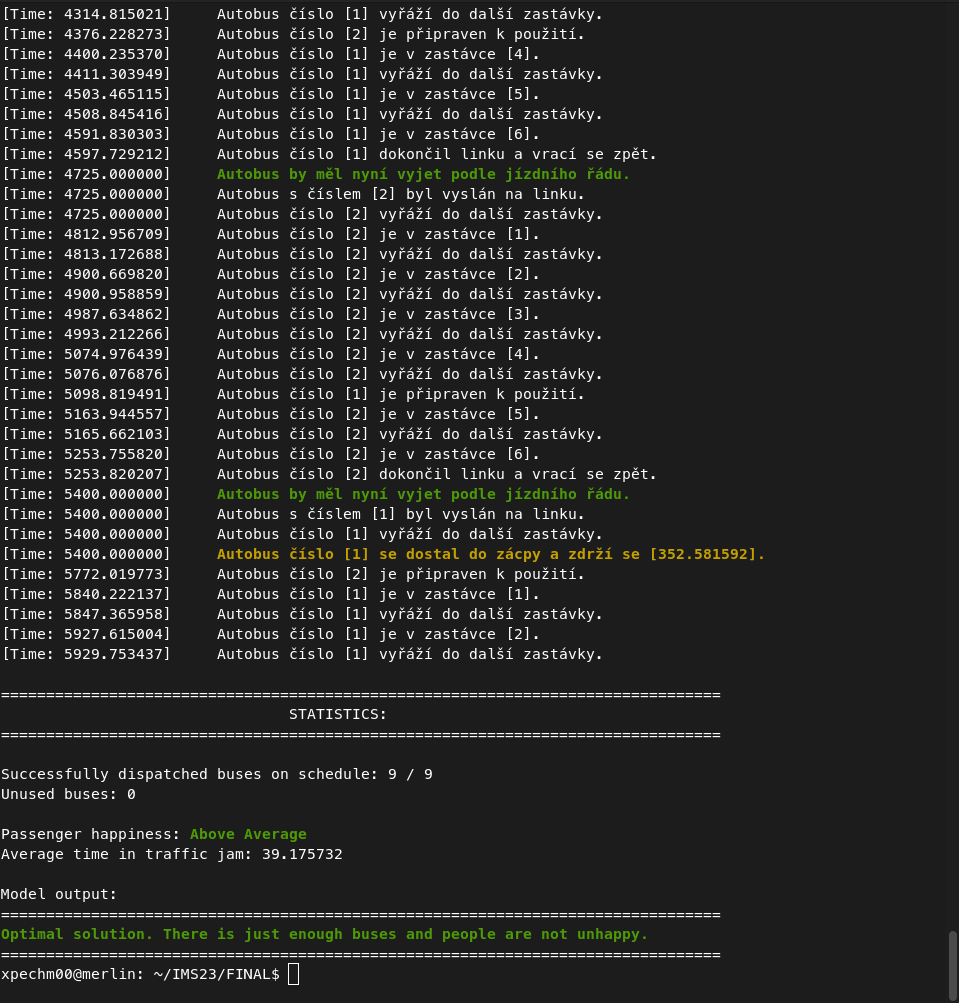
\includegraphics[scale=0.48, keepaspectratio]{fig/ims_bus3.png}
                \caption{Výsledek experimentu 3 - zkrácená linka v dopravní špičce}
                \label{fig:experiment3}
            \end{figure}
            \newpage
            \subsubsection{Experiment 4}
            \label{subsubsec:experiment4}
                V~tomto experimentu byla snaha vylepšit nezkrácenou linku mimo dopravní špičku přidáním několika autobusů se zachováním jízdního řádu. 

                \begin{table}[H]
                	\centering
                	\begin{tabular}{ | c | c |}
                		\hline
                		Počet autobusů & Spokojenost\\
                		\hline
                		\hline
                		4 & \textcolor{green}{Nadprůměrná} \\
                		\hline
                	\end{tabular}
                	\caption{Parametry experimentu 4}
                	\label{tab:experiment4}
                \end{table}

                Z~výsledků je patrné, že přidáním autobusů se nic nezlepší. Výstup pokusu upozorňuje na přebytečné množství vyhrazených autobusů.

                 \begin{figure}[H]
                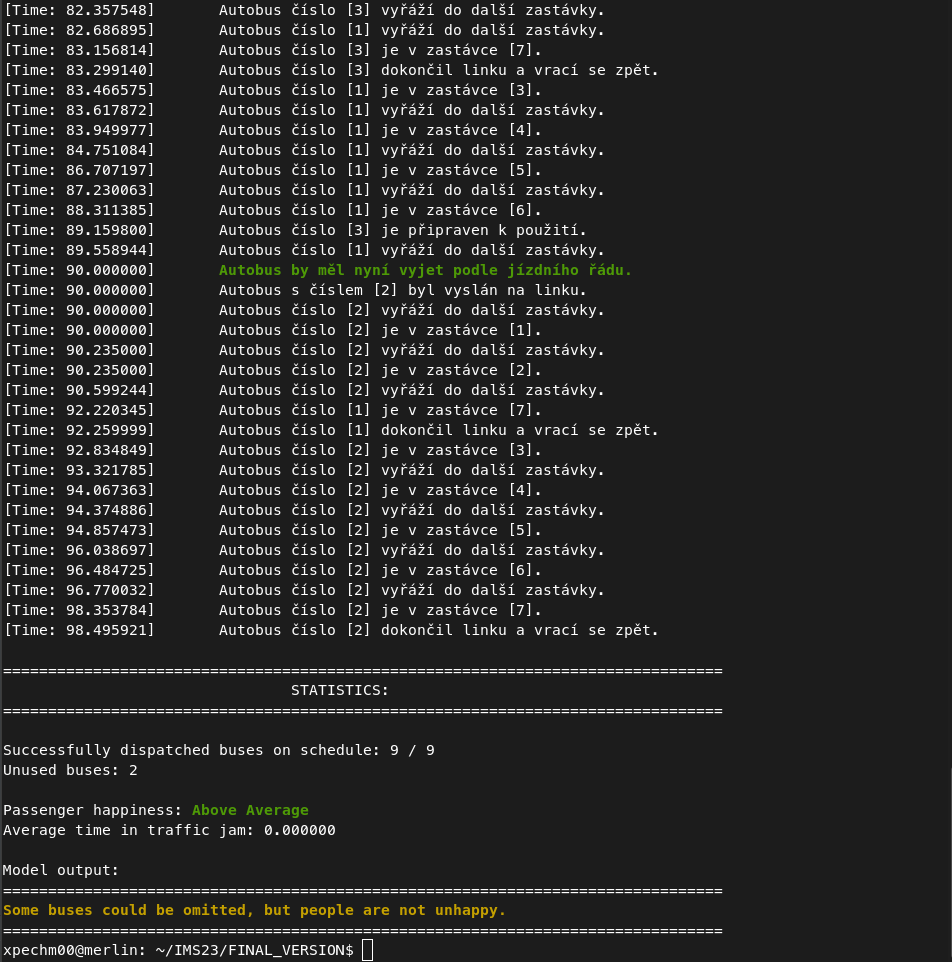
\includegraphics[scale=0.37, keepaspectratio]{fig/ims_bus4.png}
                \caption{Výsledek experimentu  - nezkrácená linka mimo špičku s přidáním několika autobusů}
                \label{fig:experiment4}
                    \end{figure}

            \newpage
            \subsubsection{Experiment 5}
            \label{subsubsec:experiment5}

                Cílem posledního experimentu bylo vyzkoušet, jak by autobusová linka fungovala, kdyby se počet autobusů na ní jezdících naopak snížil.
    
                \begin{table}[H]
                    \centering
                    \begin{tabular}{ | c | c |}
                        \hline
                        Počet autobusů & Spokojenost\\
                        \hline
                        \hline
                        2 & \textcolor{red}{Podprůměrná} \\
                        \hline
                    \end{tabular}
                    \caption{Parametry experimentu 5}
                    \label{tab:experiment5}
                \end{table}

            Dle výsledku experimentu by v situaci, kdy by za daných podmínek jezdily jen dva autobusy, byla spokojenost cestujících podprůměrná. Model doporučuje zvýšit počet autobusů, nebo snížit frekvenci s jakou autobusy jezdí (například vyslat autobus jednou za hodinu).
                
                \begin{figure}[H]
                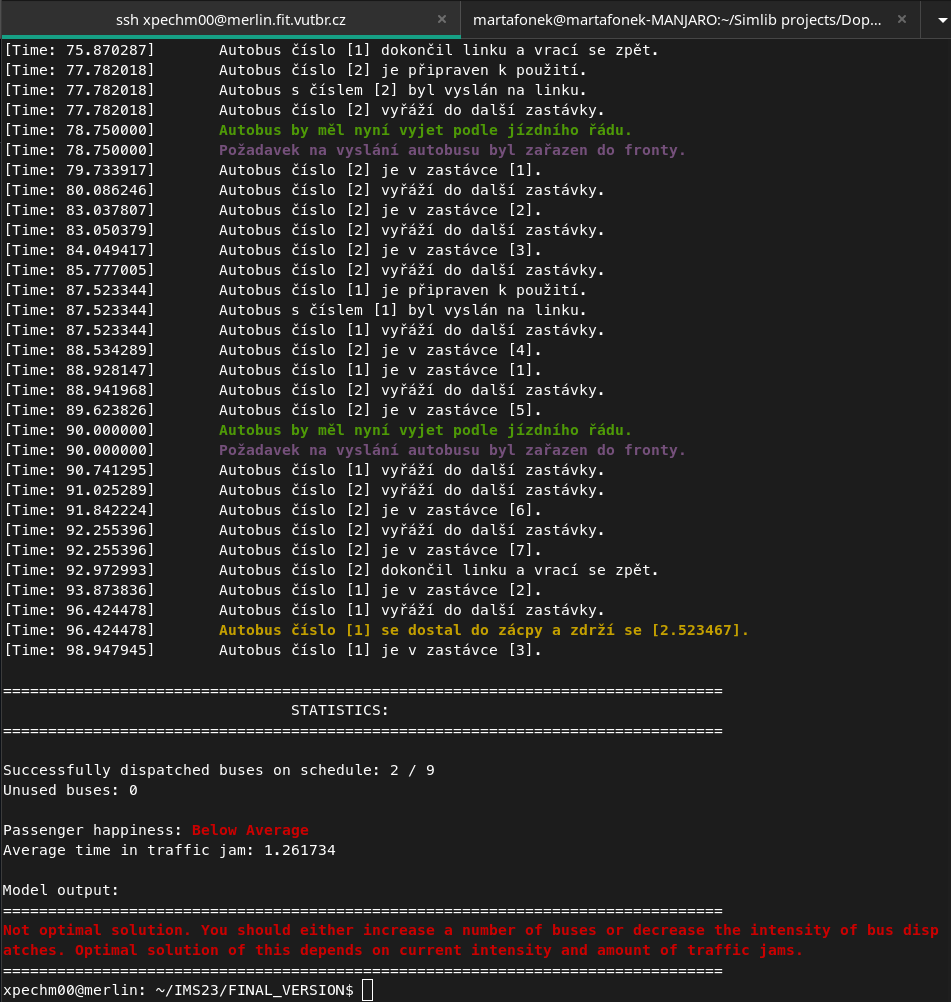
\includegraphics[scale=0.37, keepaspectratio]{fig/ims_bus5.png}
                \caption{Výsledek experimentu 5 - nízký počet autobusů}
                \label{fig:experiment5}
            \end{figure}

        \subsection{Závěry experimentů}
        \label{subsec:experiments_summary}

            Bylo provedeno 5 experimentů s~různými parametry. V prvním experimentu bylo ověřeno, že mimo dopravní špičku funguje jízdní řád autobusové linky číslo 501 optimálně. V dalších experimentech bylo testováno chování za dopravní spičky, tedy v moment, kdy cestuje více cestujících a je větší šance na vznik dopravní zácpy. Na základě experimentů bylo dosaženo závěru, že je klasický jízdní řád v době dopravní špičky nevyhovující. Na základě doporučení modelu byl navržen upravený jízdní řád, který omezuje provoz linky na úsek neobsahující místo, kde vznikají problémy s dopravou. Toto řešení se ukázalo jako optimální a odolné i v době dopravní špičky. Další experimentování mělo za cíl vyzkoušet, zdali by došlo přidáním či ubráním počtu autobusů na lince k výrazným rozdílům. V případě přidání autobusu nedošlo ke zlepšení, neboť současný počet autobusů stíhá obsloužit požadavky dostatečně dobře. V opačném případě došlo ke značnému zhoršení situace a tato varianta byla označena jako nevyhovující.
            
\newpage
    \section{Shrnutí simulačních experimentů a~závěr}
    \label{sec:summary}
    		V rámci této práce byl vytvořen nástroj, který je schopen napomáhat s tvorbou ideálních jízdních řádu a umožňuje maximalizovat efektivitu využití hromadné dopravy na konkrétní lince. Nástroj pomáhá s návrhem ideální dopravní infrastruktury, pomáhá uspokojovat potřeby cestujících a s jeho využitím může dojít ke snížení nákladů vynaložených na provoz dopravních prostředků na konkrétní lince. Funkčnost modelu byla prokázána výsledky experimentů, které korespondují s realitou.
  
    
    		V rámci experimentů byla modelu vystavena aktuální komplikovaná dopravní situace na Jihomoravské autobusové lince číslo 501. Na dané lince dochází téměř s jistotou v dopravní špičce k dopravnímu omezení kvůli rekonstrukci dálničního nájezdu. Pro správné simulování situace bylo vytvořeno několik experimentů, na jejichž základě bylo vyvozeno doporučené řešení dané situace.
            Experimenty prokázaly, že ponechání původního jízdního řádu i přes nastalou komplikaci vede k výraznému zpožďování spojů a značné nevoli přepravovaných lidí. Na základě výše uvedeného model vyhodnotil, že by bylo vhodné upravit jízdní řád, nebo navýšit počet autobusů na dané lince. Z dalších pokusů pak vyplývá, že navýšením autobusů v této situaci nedojde ke zlepšení a je třeba přistoupit k úpravám jízdního řádu.
            
            Závěr vyvozený ze skupiny pokusů doporučuje v době dopravní špičky upravit jízdní řád. Po úpravě jízdního řádu vyřazením problémového úseku model prokázal, že se komplikaci podařilo vyřešit. Vynechání tohoto úseku linky je možné z důvodu, že je na poslední zastávce před inkriminovaným místm možné přestoupit na tramvaj, kde nehrozí dopravní zácpa. Správnost tohoto řešení je podložena faktem, že se v praxi skutečně využívá výlukového jízdního řádu, který tuto situaci řeší stejným způsobem. V~rámci experimentů bylo dále ověřeno, že je aktuální jízdní řád autobusové linky číslo 501 vymyšlen dobře a měl by být odolný vůči aktuální dopravní situaci. Vzhledem k faktu, že výsledky simulace korespondují s výlukovým jízdním řádem, dal by se model považovat za validní.

 
     		Nástroj byl implementován v jazyce C++ s využitím knihovny SIMLIB. Zadáním parametrů je možné model nastavovat a modifikovat tak, aby jej bylo možné využít na řadě dalších uzlů hromadné osobní přepravy. Výstupem každého experimentu je především spokojenost cestujících, podle které je možné iterativně upravovat další parametry tak, aby bylo dosaženo ideálních výsledků. Společně se spokojeností vystupují ze simulace také podrobné statistiky, které napomáhají činit správné kroky k dosažení cíle.
			

			Nástroj by mohl být využit těmi, kteří se zaměřují na plánování spojů a linek hromadné osobní přepravy. Cílovou skupinou jsou tedy především dopravní podniky, cestovní agentury a další. Za předpokladu, že jsou do modelu vložena velmi přesná data by model mohl být velmi efektivní nástroj pro optimalizaci nákladů a určení ideálního řešení. Výsledkem použití nástroje by měla být vyšší spokojenost na straně dopravce i cestujícího.
            


    \newpage

    \renewcommand{\refname}{Použitá literatura}
    \bibliographystyle{czechiso}
    \bibliography{documentation}

\end{document}
